% !TeX root = ../../thesis.tex
\chapter{Materials and Methods}\label{ch:material_properties}

The inception of the work presented in this thesis began with the repurposing an older vacuum evaporation chamber, previously used of the fabrication of organic thin film electronics. A significant portion of initial efforts focused on calibrating the chamber for the deposition of inorganic perovskite layers, evaluating film quality and repeatability, as well as investigating the effect of fundamental deposition parameters on the performance of perovskite photodiodes. This chapter outlines the experimental protocol followed in this work, detailing the deposition and characterization methods of \ch{CsPbI_2Br} thin films, as well as the development of CMOS-imager compatible PePDs. Finally, the importance of careful interpretation of data from electrical characterization measurements is emphasized. 

\section{Thermal Co-Evaporation of \ch{CsPbI_2Br} Thin Films}

\subsection{Fundamentals}

In general terms, the process of thermal evaporation consists of three stages: 1) Vaporization: the precursor materials, which are initially in powder form, are heated up until vaporized into molecules or atoms. 2) Transportation: given that the vacuum in the chamber is high enough, the vaporized atoms/molecules transport from their source crucibles to the substrate with minimal collisions. 3) Deposition and film growth: the precursor atoms/molecules condense on the substrate, gradually nucleating to form a film \cite{Du2022ThermalOutlook}. 

The first condition for a high-quality thermal evaporation deposition is the attainment of a high vacuum in the deposition chamber. Besides the elimination of potential impurities, the vacuum level has a direct influence in the free mean path ($\lambda$) of the precursor molecules, which describes the average distance between two collisions. The relationship between $\lambda$ and vacuum pressure (P, Pa) is described by equation:

\begin{equation}
    \lambda = \frac{k_BT}{\sqrt{2}\pi d^2P},
\end{equation}

 where $k_B$ is the Boltzmann constant, $d$ is the effective molecular diameter ($\backsim 10^{-10}$ m for CsBr and \ch{PbI_2}) and T is the molecule's temperature \cite{Dong2023GrowthFilm}. Considering that the distance between source crucibles and substrate is equal to $L$, a ballistic molecule transport, i.e.  a random thermal motion of the precursors without collision processes, can be guaranteed for $\lambda >> L$. In our case, L $\approx$ 40 cm and the thermal evaporation pressure was always maintained below $\backsim 10^{-4}$~Pa, yielding a free mean path of $\lambda \approx 100$ m, satisfying the condition for ballistic transport. It has to be highlighted that this condition is only satisfied for the evaporation of inorganic precursors. Previous studies evaluated the evaporation of organic precursors (such as MAI) for the deposition of hybrid organic-inorganic perovskite thin films, however the the decomposition of MAI into more volatile compounds can lead to an up to a three order magnitude increase in background pressure, which in turn reduces the precursors' $\lambda$ \cite{Abzieher2021FromCells}.
 
 Once the molecules reach the substrate, three mechanisms of film growth are possible, namely island growth (Volmer-Weber mode), layer growth (Frank-Van der Merwe mode), and layer-island growth (Stranski-Krastanov mode) \cite{Wang2024ThermallyBeyond}. The dominant mechanism depends on adsorbate-adsorbate and adsorbate-substrate bonding strength. The prevalence of the former promotes island growth, while the dominance of the later facilitates layer growth. In the case of perovskite evaporation, the primary deposition mechanism is island growth owing to the lattice mismatch between the substrate surface and the perovskite lattice \cite{Chen2018AEfficiency}. This means that the precursor molecules nucleate on the substrate surface and grow into islands, which subsequently coalesce to form a poly-crystalline film. This initial nucleation will determine the final grain size and film morphology. Regardless of the growth mechanism, whether the precursors in situ react to form the perovskite lattice also depends on their evaporation rate and substrate temperature. The sum of the precursors' kinetic energy and substrate's thermal energy should be sufficient to surmount the reaction potential barrier for the formation of the perovskite crystal \cite{DongGrowthFilm}. 

\subsection{Process Development}


\begin{figure}
  \centering
  \medskip
  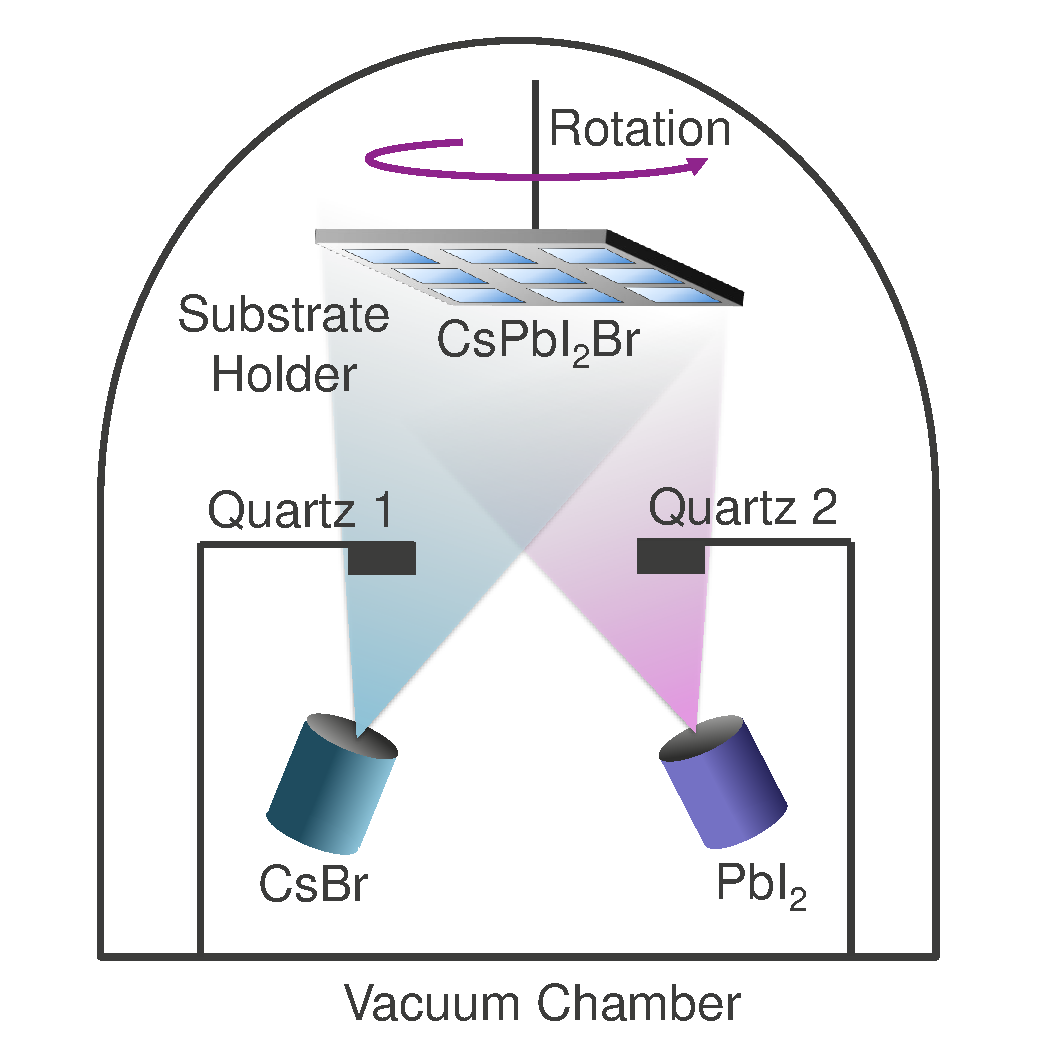
\includegraphics[width=.5\textwidth]{chapters/material_properties/images/Chamber.pdf}
  \caption[Short caption for Table of Figures]{Illustration of high-vacuum deposition chamber.}
  \label{fig:deposition_chamber}
\end{figure}


An illustration of the vacuum evaporation deposition chamber used in the scope of this thesis is provided in Figure~\ref{fig:deposition_chamber}. Two sources on opposite sides of the chamber are loaded with \ch{CsBr} and \ch{PbI_2} powders. Two separate quartz crystal microbalances (QCMs) are used to track the deposition rate of each source. The substrates are loaded on a substrate holder (approximately 40 $cm$ above the sources) that can hold up to nine $3\times 3$ $cm^2$ coupons. The QCMs have to be calibrated according to the atomic mass of the precursor they are monitoring. To achieve this, an initial estimation of their tooling factor is necessary. Subsequently, each precursor is deposited on \ch{Si/SiO_2} substrate, placed in the center of the substrate holder, and the actual thickness is measured using spectroscopic ellipsometry or profilometry. The tooling factor is then adjusted using the equation: 

\begin{equation}
    TF_{\text{actual}} = TF_{\text{approx}} \times \frac{\text{thickness(actual)}}{\text{thickness(QCM)}}
\end{equation}

To account for system variability, we deposit each precursor multiple times at different rates and target thicknesses. The final tooling factor of each source is calculated based on the average of all depositions.


Moving on to the co-evaporation of perovskite thin films, the ratio between the two sources' evaporation rates should be tuned to achieve the desired stoichiometry. For a stoichiometric film, the thickness ratio (TR) between two precursors, A and B, should be equal to: 

\begin{equation}
    TR = \frac{MolarMass(A)/Density(A)}{MolarMass(B)/Density(B)}.
\end{equation}

During the co-evaporation, a global shutter is protecting the samples while the sources are still heating up. Once both rates have reached their target value and are stabilized, the shutter is removed, initiating the deposition. The substrate holder is kept at room temperature and rotates at approximately 2.2 rounds per minute to ensure a uniform deposition. During the deposition, the temperature of each sources is continuously and automatically adjusted to maintain a constant evaporation rate. The deposition is automatically terminated once the target cumulative thickness is reached. For the development of the baseline evaporated films, a cumulative nominal deposition rate of 0.8{\AA}/s and a \ch{CsBr:PbI_2} ratio of 1.05:1.00 was aimed for. Films were deposited with a slight excess of \ch{CsBr} since it was shown that it can improve the ambient stability of the black phase without compromising their optoelectronic properties \cite{Ma2017TheCells}. Following the deposition of the perovskite thin films, they were typically flash annealed at 300 \degree C in nitrogen environment, in which they were consistently stored to prevent their conversion to the photo-inactive yellow phase. Chapter~\ref{ch:ellipsometry} will further investigate the impact of the post-deposition thermal annealing step on the material properties of the \ch{CsPbI_2Br} film.


\section{Experimental Methodology}

\begin{figure}[htbp]
    \centering
    % First plot
    \begin{subfigure}[t]{0.99\textwidth} % Adjust width as needed
        \centering
        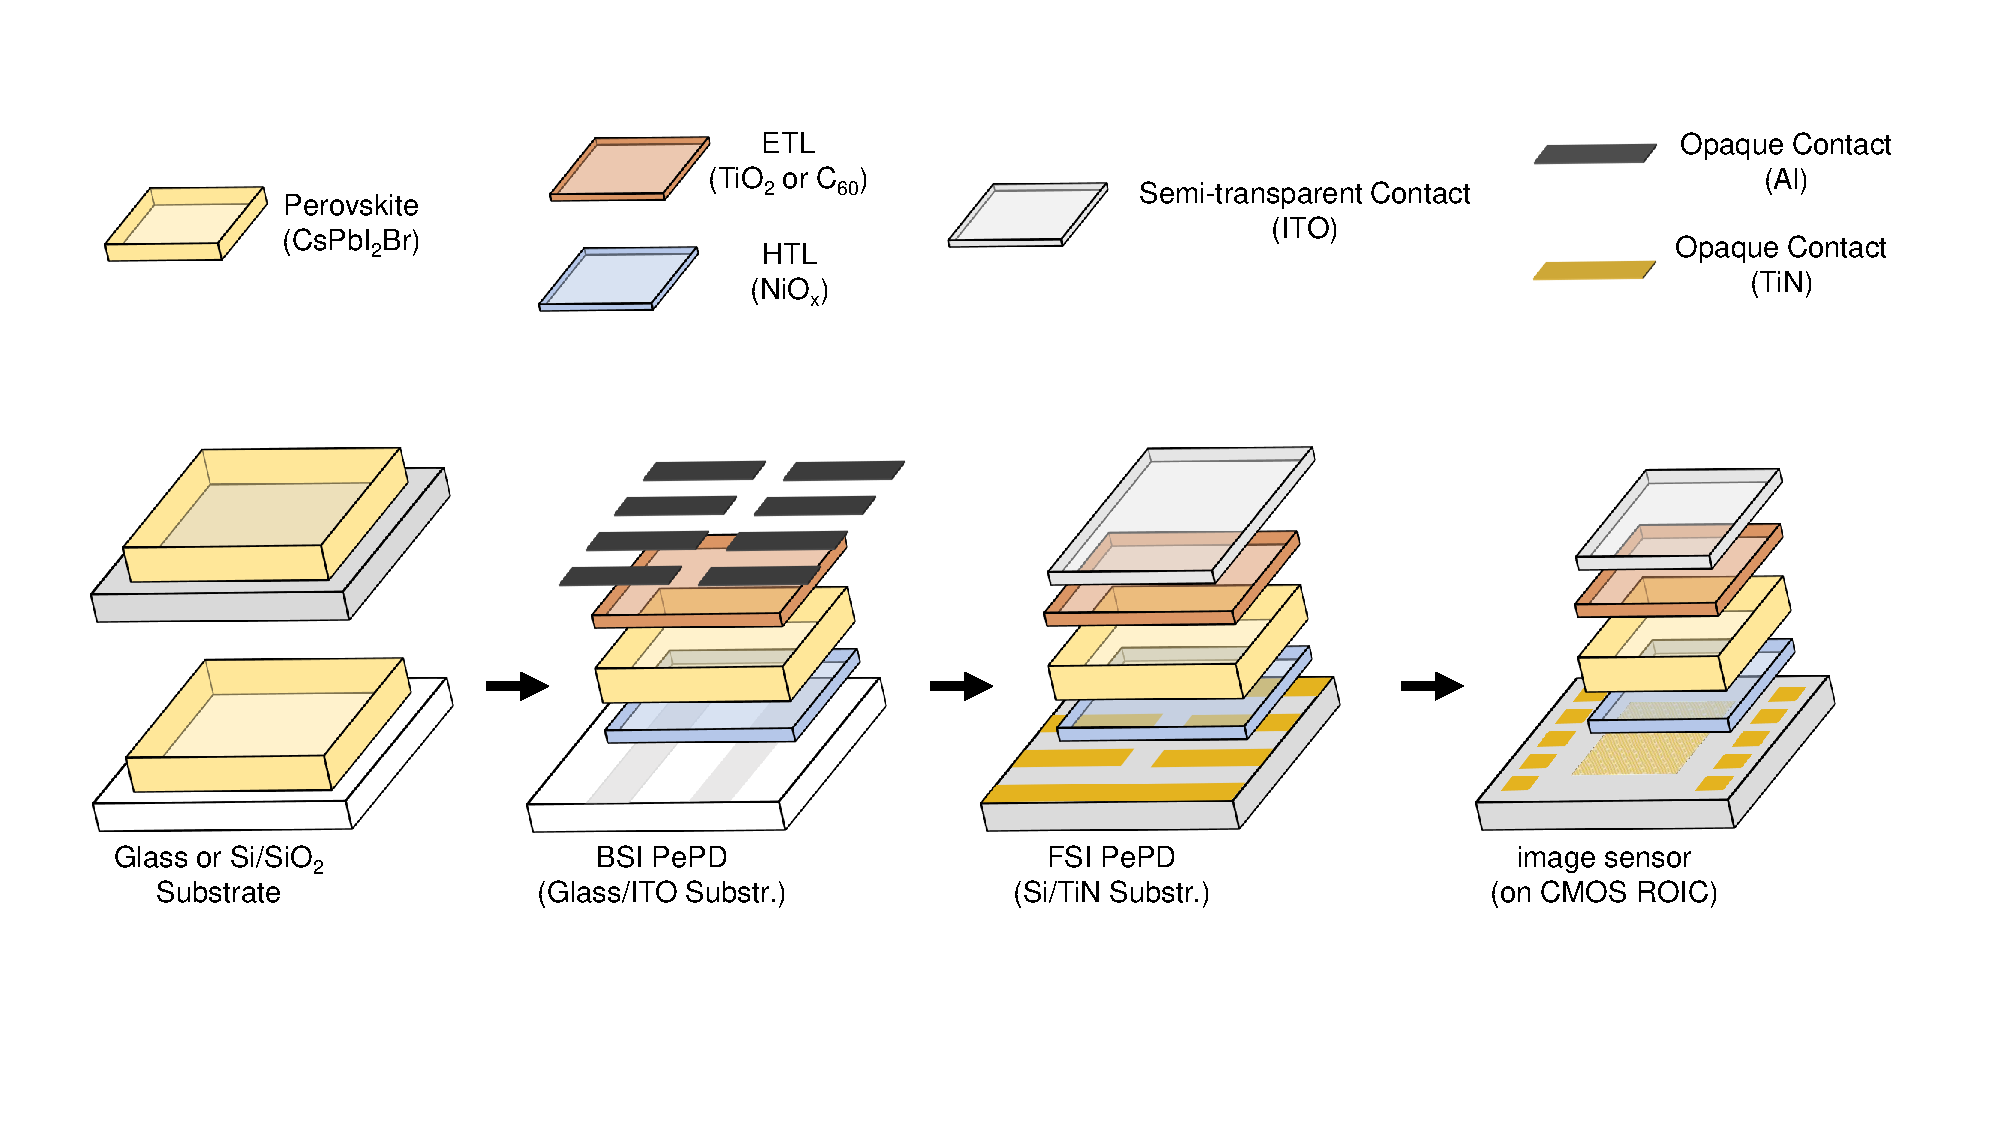
\includegraphics[width=\textwidth]{chapters/material_properties/images/methodology.pdf} % Replace with your image
    \end{subfigure}

    % Caption for the whole figure
    \caption{Methodology - Adapted from \cite{Malinowski2023ImageAbsorbers}}
    \label{fig:ch2:methodology}
\end{figure}

Once the reliable and controlled deposition of \ch{CsPbI_2Br} thin films was ensured, we followed the experimental methodology illustrated in Fig.~\ref{fig:ch2:methodology} to develop CMOS imager-compatible PePDs. The use of test structures with progressively increasing complexity allows for the efficient collection of the relevant for each structure Figures of Merit (FoM). 

Initially, the co-evaporated \ch{CsPbI_2Br} thin films are deposited on glass or Si/\ch{SiO_2} substrates, aiming to an investigation of their fundamental structural, compositional, crystallographic, and optical properties. Structural properties are mainly investigated using atomic force microscopy (AFM), scanning electron microscopy (SEM), and transmission electron microscopy (TEM). Compositional properties are inspected utilizing X-Ray and Ultraviolet photoelectron spectroscopy (XPS/UPS), energy dispersive X-Ray spectroscopy (EDS), as well as inductively coupled plasma mass spectrometry (ICP-MS). Crystallographic properties are evaluated using synchrotron-based grazing incident wide angle X-ray scattering (GIWAXS). Optical properties are investigated using photoluminescence (PL) measurements, ultraviolet-visible spectroscopy (UV-Vis), and spectroscopic ellipsometry (SE). Finally, in this initial stage of material characterization, the ambient stability of the \ch{CsPbI_2Br} black phase was assessed by exposing the films to the controlled laboratory environment and monitoring their conversion to the yellow phase over time.

After ensuring the high quality of the bare perovskite films and knowing their optical properties, they are followingly incorporated into the backside illuminated (BSI) photodiode stack, which relies on the use of glass substrates, pre-patterned with semi-transparent indium tin oxide (ITO) contacts. The perovskite thin film, sandwiched between two charge transport layers (CTLs), is deposited on the glass/ITO substrate, with the stack being completed with the deposition of a reflective top contact (Al). In this configuration, the ITO stripes serve as the diodes' common contact, while the device area is defined by the opening of the top contact shadow mask, as illustrated in Fig.~\ref{fig:ch2:types_of_substrates}a. For a total of 12 devices that are defined on the same substrate, the area of the top contacts varies between 3 values (0.125, 0.075, and 0.025 $cm^2$), allowing us to disentangle area-dependent from non-area-dependent performance characteristics. The development of BSI photodiodes has the advantage of allowing rapid prototyping and the screening of various deposition parameters/layers, considering that the supply of glass/ITO substrates was inexpensive and unlimited. The characterization of the BSI PePDs typically relies on the acquisition of J-V (in dark and under illumination), EQE, as well as capacitance and transient photocurrent measurements. This protocol allows for the identification of the optimal perovskite and CTL processing conditions that ensure the lowest $J_d$ and highest EQE (or $J_{photo}$), while ensuring device performance repeatability, optimal response speed and stability of the PePDs under the effect of reverse bias. 

\begin{figure}[htbp]
    \centering
    % First plot
    \begin{subfigure}[t]{0.49\textwidth} % Adjust width as needed
        \centering
        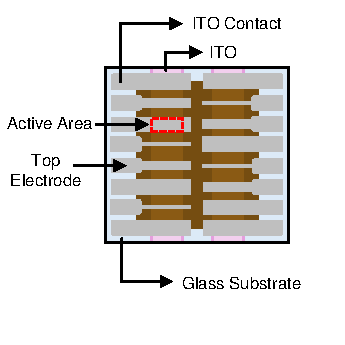
\includegraphics[width=\textwidth]{chapters/material_properties/images/Glass_Substrate.pdf} % Replace with your image
        \caption{}
        \label{fig:ch2:glass_substrate}
    \end{subfigure}
    \hfill % Space between the two plots
    % Second plot
    \begin{subfigure}[t]{0.49\textwidth} % Adjust width as needed
        \centering
        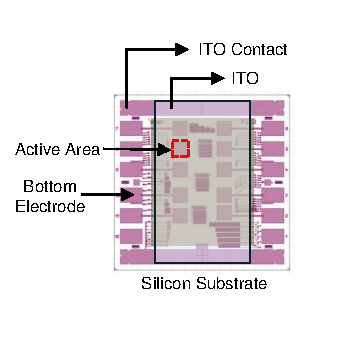
\includegraphics[width=\textwidth]{chapters/material_properties/images/PIX_Substrate.pdf} % Replace with your image
        \caption{}
        \label{fig:ch2:pix_substrate}
    \end{subfigure}

    % Caption for the whole figure
    \caption{Substrate layouts: (a) glass substrate, and (b) silicon substrate. The brown area represent the area that is covered by the perovskite and the transport layers. }
    \label{fig:ch2:types_of_substrates}
\end{figure}


Once the performance of the BSI PePDs has been optimized, the same process flow is repeated on top of a Si substrate for the fabrication of front-side illuminated (FSI) devices. The silicon substrates (shown in Fig.~\ref{fig:ch2:types_of_substrates}b), which are designed internally and fabricated in imec's CMOS foundry, are patterned with titanium nitride (TiN) contacts that define the device area (0.0625 $cm^2$). In this case, the common contact is defined by an ITO layer that is deposited on top of the PePD stack. The TiN contacts are the same as the ones found on the image sensor, albeit without the pixel circuitry below them, therefore the performance of the discrete PDs in this stage should emulate the electrical and optical properties of the target readout interface. At this stage, the same electrical characterization measurements as in the previous step are conducted, with the only difference being the direction of illumination. Even though the choice and processing of the perovskite and CTLs is the same as in the previous step, the use of different contacts and illumination direction establish certain differences that ought to be further understood and investigated. Finally, the elimination of Al from the device stack allows for the characterization of the PePD's thermal (> 250\degree C) and ambient atmosphere stability. 

The last stage, which is outside the scope of the work presented in this thesis, involves the integration of the PePD on top of the CMOS ROIC substrate (the cross-section of which was shown in Fig.~\ref{fig:ch1:cmos_roic}, which can be used to capture 2-D or 3-D images, as well as to characterize relevant parameters, related to signal conversion, spatial uniformity, and photoresponse nonuniformity \cite{Malinowski2023ImageAbsorbers, Song2024HalideImager}. 



\section{Charge Transport Layers}

\begin{figure}[htbp]
    \centering
    % First plot
    \begin{subfigure}[t]{0.35\textwidth} % Adjust width as needed
        \centering
        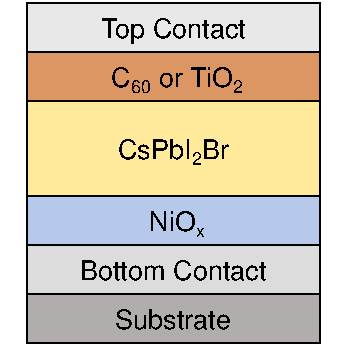
\includegraphics[width=\textwidth]{chapters/material_properties/images/stack_cross_section.pdf} % Replace with your image
        \caption{}
        \label{}
    \end{subfigure}
    \hfill % Space between the two plots
    % Second plot
    \begin{subfigure}[t]{0.45\textwidth} % Adjust width as needed
        \centering
        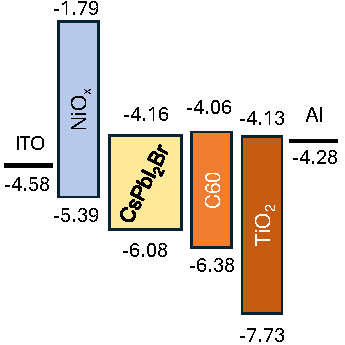
\includegraphics[width=\textwidth]{chapters/material_properties/images/energy_landscape.pdf} % Replace with your image
        \caption{}
        \label{}
    \end{subfigure}

    % Caption for the whole figure
    \caption{Stack and Energy landscape}
    \label{fig:ch2:stack_and_energy_landscape}
\end{figure}

Unlike perovskite thin films, which are predominantly deposited using solution processing techniques, the utilization of vacuum deposition methods is far more common in the case of CTLs. This is because, in solar cell research, the perovskite layer is typically hundreds of nanometers thick, allowing its deposition on large-area modules using techniques such as blade coating or inkjet printing. On the other hand, CTLs require only a few tens of nanometers in thickness, posing significant challenges for achieving uniform and conformal deposition over large areas using solution-processing methods \cite{Luo2025VacuumModules}. The most common vacuum deposition techniques that have been explored for the deposition of CTLs include magnetron sputtering (MS), thermal evaporation (TE), electron beam evaporation (EBE), chemical vapor deposition (CVD), atomic layer deposition (ALD), and pulsed layer deposition (PLD).

With the exception of TE, the rest of the aforementioned vacuum processing techniques are primarily associated with the deposition of metal oxides, most commonly including titanium oxide (\ch{TiO_2}), zinc oxide (\ch{ZnO}), tin oxide (\ch{SnO_2}), and nickel oxide (\ch{NiO_x}). The use of metal oxides automatically satisfies the condition of high-temperature tolerance that is imposed in the scope of this thesis. On the other hand, owing to its milder deposition conditions, TE allows for the utilization of a larger variety of TLs, such as \ch{C_{60}} (buckminsterfullerene), Spiro-OMeTAD (2,2',7,7'-Tetrakis[N,N-di(4-methoxyphenyl)amino]-9,9'-spirobifluorene), \ch{CuPc} (copper phthalocyanine), PTAA (Poly[bis(4-phenyl)(2,4,6-trimethylphenyl)amine), \ch{MoO_3} (molybdenum oxide), and TaTm (N4,N4,N4'',N4''-tetra([1,1'-biphenyl]-4-yl)-[1,1':4',1''-terphenyl]-4,4''-diamine). However, certain compounds, such as Spiro-OMeTAD, are know to have poor thermal stability, degrading at temperatures even below 150°C, which automatically leads to their exclusion from possible TL candidates \cite{Zhao2017EffectCells, Tumen-Ulzii2020UnderstandingTemperature, Jeong2022ChallengesCells}. 


In the scope of the work presented in this thesis, DC sputtered \ch{NiO_x} was the only HTL utilized, owing its reliable and consistent performance. Due to the harsh conditions of the sputtering process, the \ch{NiO_x} was always deposited before the perovskite layer, independently of the substrate used (glass or silicon). The films were deposited via reactive sputtering of a metallic nicker target, using oxygen plasma. Post-deposition, the substrates would be annealed in open air for 5 minutes at 300 \degree
C to reduce oxygen vacancies and increase the film's transparency. In terms of the ETL, the use of e-beam deposited \ch{TiO_2} and thermally-evaporated \ch{C_{60}} was evaluated. The cross-section of the developed PePD stack, as well as the energy levels of the constituent layers are indicated in Fig.~\ref{fig:ch2:stack_and_energy_landscape}a and b, respectively. Chapter~\ref{ch:transport_layer} will discuss in detail the influence of the ETL on the PePD's performance and reliability. 


\section{Impact of Characterization Method and Statistical Remarks}



The electrical characterization of perovskite-based devices is not a straight-forward task, as their performance is influenced by both electronic and ionic mechanisms. A direct consequence of this feature is the presence of hysteresis in J-V measurements, which has been shown to depend not only on the scan's direction and speed, but also on the composition of the perovskite layer and the choice of transport layers \cite{Snaith2014AnomalousCells,Dualeh2014ImpedanceCells}.
The underlying cause behind such phenomena is a complex matrix of mechanisms that involves the generation, transport and annihilation of ionic defects, which is usually, simplistically, referred to as "ion migration" \cite{Xu2024BeyondPerspective}. During characterization under dark conditions, the generation of ionic defects is typically attributed to electrochemical reduction/oxidation (redox) mechanisms, such as the oxidation of the iodide anions into iodine interstitials and halide vacancies. These mobile ions and defects may further undergo reversible or irreversible reactions to a achieve a lower energy state. Some aftermaths of such  reactions might include phase segregation in mixed halide perovskites, the doping of organic HTLs or the formation of metal filaments \cite{Kerner2021OrganicDevices, Hoke2014ReversiblePhotovoltaics,Xu2023Reverse-biasCells}. The electric bias applied during a J-V scan is sufficient to promote the generation and transport of ionic defects, thus making it challenging to disentangle phenomena attributed to charge carriers, mobile ions, or newly formed species within the perovskite layer. 

The presence of hysteresis in sequential J-V scans is quite dominant during the characterization of the PePDs developed in the framework of this thesis, as revealed in Fig.~\ref{fig:ch2:scan_direction} and Fig.~\ref{fig:ch2:scan_speed}, which examine the impact of scan direction and integration time, respectively. With the potential causes of this behavior ranging from the phase-segration-prone nature of the \ch{CsPbI_xBr_{3-x}} composition, the contribution of abundant grain boundaries to the generation/transport of mobile ions or the dubious role of the CTLs and metal contacts, it is impossible to pinpoint the exact origins of hysteresis in the J-V data \cite{Ghasemi2023APerovskites, Shao2016GrainFilms, Yun2016CriticalCells, Meggiolaro2019FormationPerovskites, Aristidou2017FastCells, Barker2017Defect-AssistedFilms,Li2018InorganicCells,Ighodalo2023NegligiblePerovskites}. One thing that becomes clear, however, is that defining key figures of merit, such as $J_d$, is not straightforward and should always be considered within the context of characterization settings.

\begin{figure}[ht!]
    \centering

    % First row
    \begin{subfigure}[b]{0.35\textwidth}
        \centering
        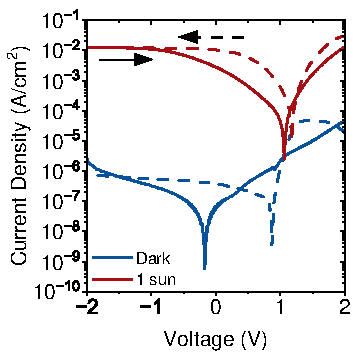
\includegraphics[width=\textwidth]{chapters/material_properties/images/Forward-Reverse-Plot.pdf}
        \caption{}
        \label{fig:ch2:scan_direction}
    \end{subfigure}
    \hspace{1cm} % Adjust this value to bring them closer
    \begin{subfigure}[b]{0.35\textwidth}
        \centering
        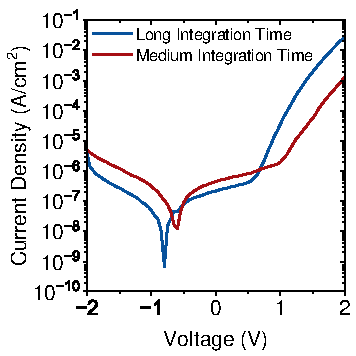
\includegraphics[width=\textwidth]{chapters/material_properties/images/Integration-Speed.pdf}
        \caption{}
        \label{fig:ch2:scan_speed}
    \end{subfigure}

    % Second row
    \begin{subfigure}[b]{0.3\textwidth}
        \centering        
        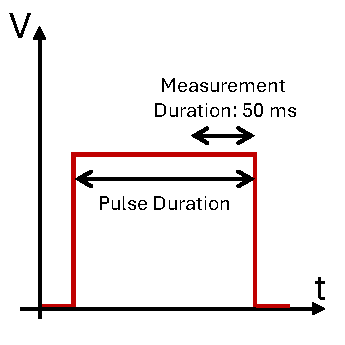
\includegraphics[width=\textwidth]{chapters/material_properties/images/PAIOS_Pulsed_Measurement.pdf}
        \caption{}
        \label{fig:ch2:pulsed_meas_PAIOS}
    \end{subfigure}
    \hspace{1cm} % Adjust spacing
    \begin{subfigure}[b]{0.35\textwidth}
        \centering
        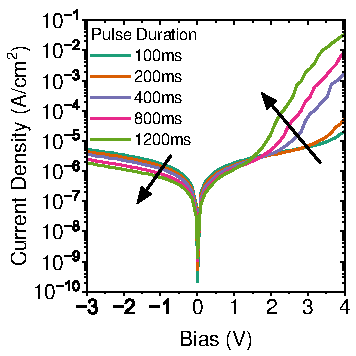
\includegraphics[width=\textwidth]{chapters/material_properties/images/Pulsed-PAIOS-plot.pdf}
        \caption{}
        \label{fig:ch2:pulsed_paios}
    \end{subfigure}

    % Third row - Centered figure
    \begin{subfigure}[b]{0.35\textwidth}
        \centering
        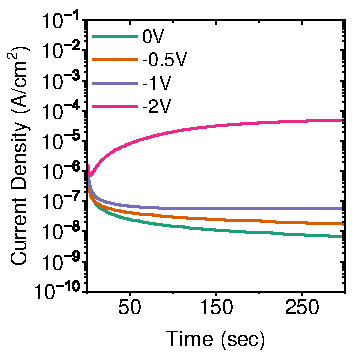
\includegraphics[width=\textwidth]{chapters/material_properties/images/Steady-State-plot.pdf}
        \caption{}
        \label{fig:ch2:steady_state}
    \end{subfigure}

    \caption{Impact of characterization methodology on device performance}
    \label{fig:ch2:types_of_measurement}
\end{figure}


One possible way of eliminating hysteresis in J-V data, is by employing a pulsed J-V measurement,
the principle of which is demonstrated in Fig.~\ref{fig:ch2:pulsed_paios}. Specifically, each voltage step is applied as a pulse of specific length (pulse duration). The current value for each voltage step is then extracted as the average transient current during a measurement of specified duration at the end of the voltage pulse. This approach allows the mobile ions to re-distribute for each voltage step, eliminating the hysteresis from the J-V data (minimum $J_d$ is at 0 V, as shown in Fig.~\ref{fig:ch2:pulsed_meas_PAIOS}). However, even for this type of measurement, it is clear that the duration of each voltage pulse has a major impact on the measured J-V performance, with longer pulses leading to lower values of $J_d$ and higher rectification in the forward bias regime. A last option for the characterization of the perovskite-based photodiodes is steady-state measurements, where a constant bias is applied and maintained for a prolonged period (300 seconds), until the value of monitored current starts saturating. This is demonstrated in Fig.~\ref{fig:ch2:steady_state}. A large drop in the value of $J_d$ is observed within the first seconds of the measurement, which was previously shown to depend on capacitive effects, rather than the presence of mobile ions \cite{Ollearo2021UltralowGeneration}. At -2 V, an almost 3-order increase in $j_d$ is observed, which has been associated with the breaking down of the device. This mechanism is concealed when performing J-V scans of relatively small duration and will be further investigated in Chapter~\ref{ch:transport_layer}. 

Considering the variability of results based on the characterization settings, we adopt the following methodology for characterizing our PePDs: sequential J-V scans in the forward direction (from reverse to forward biasing conditions) were initially utilized for the preliminary comparison of various stacks and processing conditions. Once the most promising candidates were identified, a more elaborate characterization was performed using steady-state measurements.  


\begin{figure}[htbp]
    \centering
    % First plot
    \begin{subfigure}[t]{0.4\textwidth} % Adjust width as needed
        \centering
        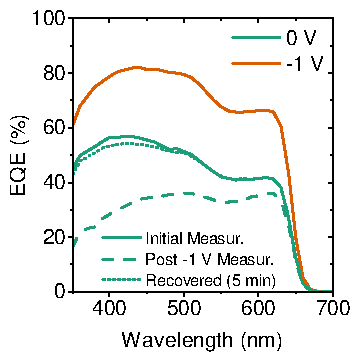
\includegraphics[width=\textwidth]{chapters/material_properties/images/EQE-1V.pdf} % Replace with your image
        \caption{}
        \label{fig:ch2:eqe-1V}
    \end{subfigure}
    \hfill % Space between the two plots
    % Second plot
    \begin{subfigure}[t]{0.4\textwidth} % Adjust width as needed
        \centering
        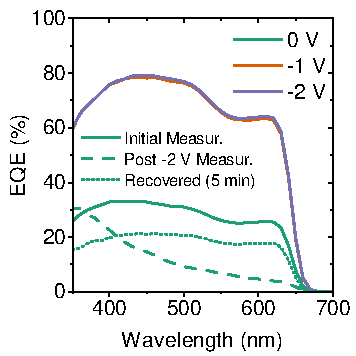
\includegraphics[width=\textwidth]{chapters/material_properties/images/EQE-2V.pdf} % Replace with your image
        \caption{}
        \label{fig:ch2:eqe-2V}
    \end{subfigure}

    
    \begin{subfigure}[t]{0.9\textwidth}
        \centering
        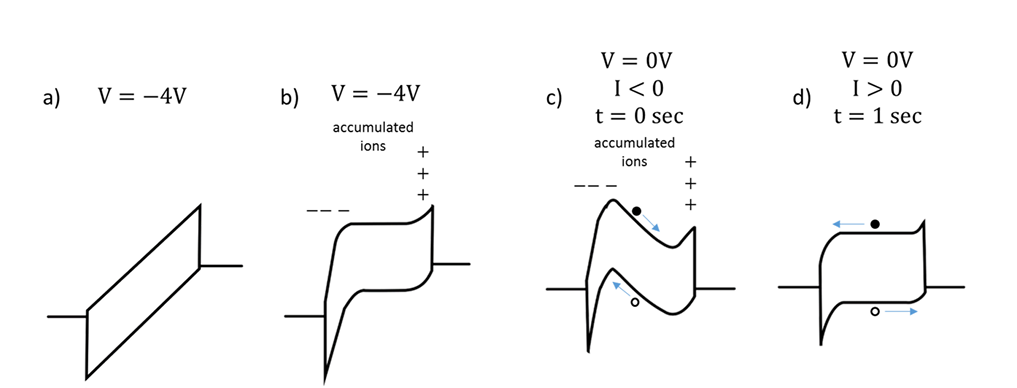
\includegraphics[width=\textwidth]{chapters/material_properties/images/ions.png} % Replace with your image file
        \caption{}
        \label{fig:ch2:eqe_drop_mechanism}
    \end{subfigure}

    % Caption for the whole figure
    \caption{Impact of measurement order on the EQE measurements.}
    \label{fig:ch2:eqe}
\end{figure}

The impact of the characterization approach on the acquired results extends to EQE measurements, as well. Fig.~\ref{fig:ch2:eqe-1V} and \ref{fig:ch2:eqe-2V} demonstrate the EQE results for two different devices that were fabricated on the same substrate. The EQE of the first device was measured sequentially at 0 V and -1 V, while the second device underwent measurements at 0 V, -1 V, and -2 V. Following these measurements, each device was subjected to two additional EQE measurements at 0 V: one immediately after the highest applied reverse bias (-1 V and -2 V, respectively) and another after a five-minute resting period in the dark. For both devices, the EQE at 0 V immediately after reverse biasing was significantly lower than the initial EQE measurement at 0 V. However, for the device biased up to -1 V, a five-minute resting period was sufficient to fully restore the initial EQE value. In contrast, for the device biased up to -2 V, the EQE at 0 V remained approximately 40\% lower than its initial value even after five minutes of recovery. This phenomenon could potentially be attributed to the mechanism that is introduced in Fig.~\ref{fig:ch2:eqe_drop_mechanism}, where the ions accumulate in response to the applied electric field (-4 V in the case of the example), so when the external bias is removed (0 V) they create a field that opposes the extraction of photo-generated carriers until they redistribute within the perovskite lattice. However, theoretical and experimental calculations estimate that the ionic field should recover withing one second \cite{Bowring2018ReverseCells}. Therefore, this mechanism cannot fully explain the reduced EQE response we observe at 0 V, even after 5 minutes of resting in the dark. In the contrary, it indicates the presence of a slower mechanism, such as the redox reactions that were discussed earlier, whose rate depends on the applied bias (hence the difference between applying -1 and -2 V). This experiment further highlights the sensitivity of acquired results on prior biasing conditions. For this reason, the EQE results presented in this work are always measured on new devices, without prior biasing, and conducted from the lowest to the highest reverse bias conditions.


\begin{figure}[ht!]
    \centering
    % First row
    \begin{subfigure}[t]{0.4\textwidth}
        \centering
        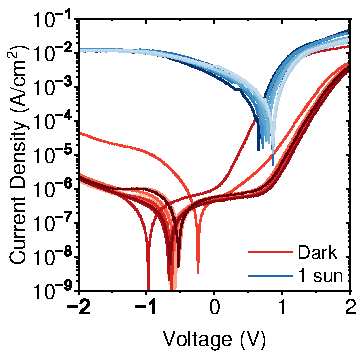
\includegraphics[width=\textwidth]{chapters/material_properties/images/High_yield_discrete.pdf} 
        \caption{}
        \label{fig:ch2:high_yield_discrete}
    \end{subfigure}
    \hfill
    \begin{subfigure}[t]{0.4\textwidth}
        \centering
        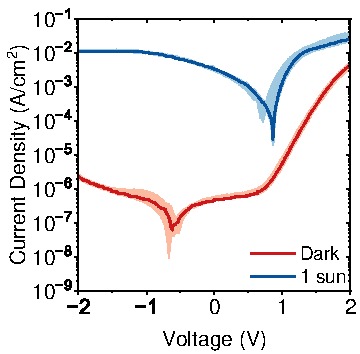
\includegraphics[width=\textwidth]{chapters/material_properties/images/High_yield_median.pdf} % Replace with your image file
        \caption{}
        \label{fig:ch2:high_yield_median}
    \end{subfigure}

    \vspace{1em} % Space between rows

    % Second row
    \begin{subfigure}[t]{0.4\textwidth}
        \centering
        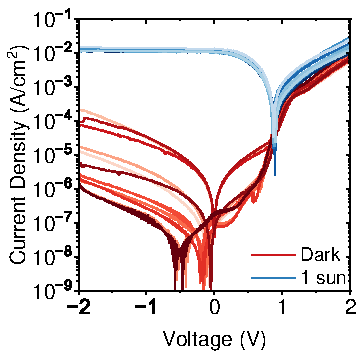
\includegraphics[width=\textwidth]{chapters/material_properties/images/low_yield_discrete.pdf} % Replace with your image file
        \caption{}
        \label{fig:ch2:low_yield_discrete}
    \end{subfigure}
    \hfill
    \begin{subfigure}[t]{0.4\textwidth}
        \centering
        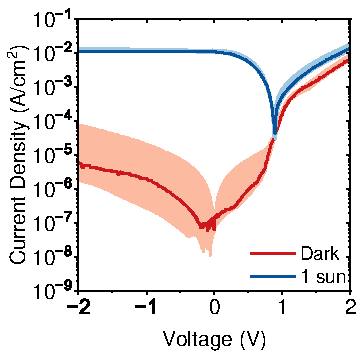
\includegraphics[width=\textwidth]{chapters/material_properties/images/low_yield_median.pdf} % Replace with your image file
        \caption{}
        \label{fig:ch2:low_yield_median}
    \end{subfigure}
    \caption{Discrete and statistical representation of J-V curves for samples with high and low variability. Reproduced from \cite{Bowring2018ReverseCells}}
    \label{fig:ch2:discrete_and_median}
\end{figure}


Another important remark is related to the fair representation of J-V data across the 12 devices that are typically fabricated on the same substrate. The relatively large device areas (0.025 $cm^2$ - 0.125 $cm^2$ for glass substrates and 0.0625 $cm^2$ for silicon substrates) increase the likelihood of faulty devices due to defects or process variations. The number and distribution of outliers determine the variability in the sample's performance. For this reason,
we employ a statistical representation of J-V data, providing the median value and interquartile range for each bias point. The discrete and statistical J-V representation for a sample with small and large variability is illustrated in Fig.~\ref{fig:ch2:discrete_and_median}a-b and Fig.~\ref{fig:ch2:discrete_and_median}c-d, respectively. This approach allows for distinguishing between stochastic defects (such as scratches or dust particles that may introduce one or two outliers) and systematic defects that lead to large variability and may be attributed to the selected materials or processing conditions. 


Lastly, it is important to address the repeatability and reliability of the PePDs fabricated in this thesis. The results presented in the following chapters correspond to devices that exhibited reproducible and consistent behavior across multiple experimental runs. However, the fabrication tools used in this study were shared across various activities within the group, sometimes experiencing periods of downtime or non-standard behavior. Consequently, fabricating an identical PePD stack in the 2nd and 4th year of the PhD may have occasionally resulted in slight variations in device performance. Given the numerous variables in a lab environment, pinpointing the exact causes of these variations becomes challenging. This is mentioned to highlight that, in the present work, only samples fabricated within close temporal proximity are compared in order to ensure meaningful conclusions, based on devices prepared under similar processing conditions.

 


%%%%%%%%%%%%%%%%%%%%%%%%%%%%%%%%%%%%%%%%%%%%%%%%%%
% Keep the following \cleardoublepage at the end of this file, 
% otherwise \includeonly includes empty pages.
\cleardoublepage

